% !TeX spellcheck = pt_BR
\documentclass[tese_patricia]{subfiles}
\begin{document}

% ---------------------------------------------------------- 
% Métodos de malhas sobrepostas
% ----------------------------------------------------------
\chapter[Dinâmica dos sólidos computacional]{Dinâmica dos sólidos computacional} \label{capitulo:Cap3}
% ----------------------------------------------------------

Assim como no caso da Mecânica dos Fluidos, um sólido é modelado considerando-o como um corpo contínuo, e seu movimento é governado também por um conjunto de equações provenientes das leis de: conservação da quantidade de movimento, conservação da massa e conservação da energia. Entretanto, diferentemente dos fluidos, os sólidos possuem resistência a esforços normais e tangenciais até que alcancem seu limite resistente, e por isso, apresentam deslocamentos e deformações finitos. Sendo os deslocamentos, ou posições atuais ao longo do tempo, as variáveis de interesse na resolução do conjunto de equações que descrevem seu comportamento. Por esse motivo, uma descrição do tipo Lagrangiana é mais adequada para essas análises.

Com respeito à escala de deslocamentos e de deformação, os sólidos podem apresentar comportamento linear ou não-linear, sendo as não linearidades de natureza geométrica (unicamente devidas à escala de deslocamentos) ou física (mudanças na relação constitutiva do material). 

Ao se tratar de problemas elásticos com grandes deslocamentos, apenas as não linearidades geométricas são levadas em consideração, e em relação ao problema linear, altera-se a forma com que se considera o equilíbrio das forças no sólido. Em uma modelagem linear, onde um corpo sofre pequenos deslocamentos e deformações, o equilíbrio é realizado em relação a configuração inicial (que é muito próxima da atual). Já em uma análise não-linear, ver com mais detalhes os trabalhos de \citeonline{Ogden:1984} e \citeonline{Coda:2018}, o equilíbrio é considerado na configuração atual.

Nesse estudo, é utilizada uma análise não-linear geométrica, visto que, em muitos problemas de IFE, como \textit{flutter} e \textit{buffeting}, grandes deslocamentos estão envolvidos. Além disso, o sólido é descrito na forma Lagrangiana Total, e considera-se o equilíbrio dinâmico do mesmo. 

A solução numérica é obtida através do método dos elementos finitos em abordagem posicional \cite{Coda:2003,Coda:2018}, onde as variáveis principais são as posições nodais. Escolhe-se trabalhar com elementos de cascas, uma vez que esses podem representar a maioria dos problemas estruturais 3D. No casos das cascas são adicionadas às incógnitas nodais vetores generalizados e um termo de que considera a variação linear da espessura do elemento para permitir o mapeamento completo do sólido. 

\begin{comment}
\nomenclature[D,01]{$\Omega_{x}$}{Domínio inicial de um sólido deformável;}
\nomenclature[D,02]{$\lPosition$}{Coordenadas ou posições materiais do domínio inicial;}
\nomenclature[D,03]{$\Omega_{y}$}{Domínio atual de um sólido deformável;}
\nomenclature[D,04]{$\ePosition$}{Coordenadas ou posições espaciais do domínio atual;}
\nomenclature[D,05]{$\deformation$}{Função mudança de configuração para um descrição Lagrangiana;}
\nomenclature[D,06]{$\greenStrain$}{Tensor de deformações de Green-Lagrange;}
\nomenclature[D,07]{$\cauchyStretch$}{Tensor de alongamento à direita de Cauchy-Green;}
\nomenclature[D,08]{$\gradDeformation$}{Grandiente da função mudança de configuração;}
\nomenclature[D,09]{$\mathbf{u}$}{Vetor qualquer definido na configuração inicial;}
\nomenclature[D,10]{$\mathbf{v}$}{Vetor qualquer definido na configuração atual;}
\nomenclature[D,11]{$dV_{0}$}{Infinitésimo de volume definido na configuração inicial;}
\nomenclature[D,12]{$dV$}{Infinitésimo de81 volume definido na configuração atual;}
\nomenclature[D,13]{$\mathbf{dx}^{i}$}{Vetor que define o lado $i$ de um infinitésimo de volume na configuração inicial, com $i = 1,2,3$;}
\nomenclature[D,14]{$dx_{j}^{i}$}{Componente do vetor $mathbf{dx}^{i}$ na direção do eixo $x_{j}$;}
\nomenclature[D,15]{$\mathbf{dy}^{i}$}{Vetor que define o lado $i$ de um infinitésimo de volume na configuração atual, com $i = 1,2,3$;}
\nomenclature[D,16]{$dy_{j}^{i}$}{Componente do vetor $mathbf{dy}^{i}$ na direção do eixo $y_{j}$;}
\nomenclature[D,17]{J}{Jacobiano da transformação, definido como $det(\gradDeformation)$};
\nomenclature[D,18]{$\mathbf{dA}_{0}$}{Vetor de área da seção transversal de um volume na configuração inicial;}
\nomenclature[D,19]{$\mathbf{dA}$}{Vetor de área da seção transversal de um volume na configuração atual;}
\nomenclature[D,20]{$\mathbf{N}$}{Vetor normal a uma superfície na configuração inicial;}
\nomenclature[D,21]{$\mathbf{n}$}{Vetor normal a uma superfície na configuração atual;}
\nomenclature[D,22]{${dA}_{0}$}{Área da seção transversal de um volume na configuração inicial;}
\nomenclature[D,23]{${dA}$}{Área da seção transversal de um volume na configuração atual;}
\nomenclature[D,24]{$\mathbf{B}$}{Tensor definido como $\mathbf{B} = \gradDeformation^{-t}$;}
\nomenclature[D,25]{$\extEnergy$}{Energia potencial das forças externas;}
\nomenclature[D,26]{$\intEnergy$}{Energia de deformação;}
\nomenclature[D,27]{$\kinEnergy$}{Energia cinética;}
\nomenclature[D,28]{$\totalEnergy$}{Energia total mecânica;}
\nomenclature[D,29]{$\delta(\bullet)$}{Variação aplicada a variável $(\bullet)$;}
\nomenclature[D,30]{$\ebodyLoad$}{Forças de corpo na configuração atual;}
\nomenclature[D,31]{$\tractionLoad$}{Forças de superfície na configuração atual;}
\nomenclature[D,32]{$\stresstensor$}{Tensor de tensões de Cauchy;}
\nomenclature[D,33]{$\rho$}{Massa específica do sólido;}
\nomenclature[D,34]{$\solidAccel$}{Aceleração do sólido;}
\nomenclature[D,35]{$\strainratetensor$}{Tensor de deformação linear de engenharia;}
\nomenclature[D,36]{$M$}{Massa de um corpo;}
\nomenclature[D,37]{$t$}{Instante de tempo qualquer da análise;}
\nomenclature[D,38]{$\rho_{0}$}{Massa específica do corpo na configuração inicial;}
\nomenclature[D,39]{$\ebodyLoad^{0}$}{Forças de corpo na configuração inicial;}
\nomenclature[D,40]{$\mathbf{P}$}{Tensor de tensões de Piola Kirchhoff;}
\nomenclature[D,41]{$\tractionLoad^{0}$}{Forças de superfície na configuração inicial;}
\nomenclature[D,42]{$\piolaStress$}{Segundo tensor de tensões de Piola Kirchhoff;}
\nomenclature[D,43]{$u_{e}$} {Expressão generalizada da energia de deformação;}
\nomenclature[D,44]{$\constitutiveTensor$}{Tensor constitutivo elástico isotrópico;}
\nomenclature[D,45]{$\bulkModulus$}{Módulo volumétrico;}
\nomenclature[D,46]{$\shearModulus$}{Módulo de cisalhamento;}
\nomenclature[D,47]{$\elasticModulus$ }{Módulo de elasticidade;}
\nomenclature[D,48]{$\poisonsRatio$}{Coeficiente de Poisson;}
\nomenclature[D,49]{$\deformation^{m0}$}{Função mudança de configuração da superfície média de uma casca que mapeia o domínio paramétrico para o domínio inicial;}
\nomenclature[D,50]{$\lPosition^{m}$}{Posições da superfície média de uma casca na configuração inicial;}
\nomenclature[D,51]{$\bm{\xi}$}{Coordenadas adimensionais que definem o espaço paramétrico}
\nomenclature[D,52]{$\mathbf{X}$}{Posições discretas nodais de um elemento de casca na configuração inicial;}
\nomenclature[D,53]{$N$}{Funções de forma}
\nomenclature[D,54]{$\deformation^{m1}$}{Função mudança de configuração da superfície média de uma casca que mapeia o domínio paramétrico para o domínio atual;}
\nomenclature[D,55]{$\ePosition^{m}$}{Posições da superfície média de uma casca na configuração atual;}
\nomenclature[D,56]{$\SolidPos$}{Posições discretas nodais de um elemento de casca na configuração atual;}
\nomenclature[D,57]{$\mathbf{v}^{0}$}{Vetor posição definido a partir da superfície média da casca em sua configuração inicial;}
\nomenclature[D,58]{$\mathbf{v}^{1}$}{Vetor posição definido a partir da superfície média da casca em sua configuração atual;}
\nomenclature[D,59]{$h_{0}$}{Espessura média inicial de um elemento de casca;}
\nomenclature[D,60]{$\mathbf{V}^{0}$}{Vetor posição discreto nodal na configuração inicial;}
\nomenclature[D,61]{$\mathbf{V}^{1}$}{Vetor posição discreto nodal na configuração atual;}
\nomenclature[D,62]{$\alpha$}{Taxa linear de variação da espessura de um elemento de casca;}
\nomenclature[D,63]{$\Lambda$}{Taxa linear discreta nodal da variação da espessura de um elemento de casca;}
\nomenclature[D,64]{$\deformation^{0}$}{Função mudança de configuração de uma casca que mapeia o domínio paramétrico para o domínio inicial;}
\nomenclature[D,65]{$\deformation^{1}$}{Função mudança de configuração de uma casca que mapeia o domínio paramétrico para o domínio atual;}
\nomenclature[D,66]{$\mathbf{F}$}{Vetor de forças nodais aplicadas na configuração inicial;}
\nomenclature[D,67]{$\gradDeformation^{1}$}{Gradiente da função mudança de configuração $\deformation^{1}$;}
\nomenclature[D,68]{$\gradDeformation^{0}$}{Gradiente da função mudança de configuração $\deformation^{0}$;}
\nomenclature[D,69]{$\mathbf{B}^{0}$}{Vetor discreto nodal que define as forças de corpo na configuração inicial;}
\nomenclature[D,70]{$\mathbf{Q}^{0}$}{Vetor discreto nodal que define as forças de superfície na configuração inicial;}
\nomenclature[D,71]{$\mathbf{\ddot{Y}}$}{Vetor discreto nodal que define a aceleração;}
\nomenclature[D,72]{$\concLoad^{ext}$}{Vetor discreto nodal que define as forças externas atuantes em um sólido;}
\nomenclature[D,73]{$\solidMass$}{Matriz de massa de um elemento;}
\nomenclature[D,74]{$\concLoad^{int}$}{Vetor discreto nodal que define as forças internas atuantes em um sólido;}
\nomenclature[D,75]{$\solidDamping$}{Matriz de amortecimento de um elemento;}
\nomenclature[D,76]{$\SolidVel_{}$}{Vetor discreto nodal que define a velocidade;}
\nomenclature[D,77]{$t_{n+1}$}{Tempo discreto no instante atual;} 
\nomenclature[D,78]{$t_{n}$}{Tempo discreto no instante anterior;} 
\nomenclature[D,79]{$\Delta t$}{Intervalo de tempo da discretização temporal;}
\nomenclature[D,80]{$\beta$}{Parâmetro da aproximação temporal de Newmark;}
\nomenclature[D,81]{$\gamma$}{Parâmetro da aproximação temporal de Newmark;}
\nomenclature[D,82]{$\mathbf{Q}_n$ e $\mathbf{R}_n$}{Termos da aproximação de Newmark que relacionam velocidade, aceleração e posições em um instante de tempo anterior;}
\nomenclature[D,83]{$\NNSS$}{Vetor discreto que representa o resíduo da equação de equilíbrio discretizada no espaço e tempo;}

\end{comment}

\section{Cinemática dos corpos deformáveis}

Um sólido deformável quando sujeito à ações externas, sofre uma mudança de configuração. Na Fig. \ref{fig:CinSol}, pode-se observar um sólido na sua configuração inicial $\Omega_{x}$, com suas coordenadas materiais descritas por $\lPosition$, que em outro instante, se transforma no domínio representado por $\Omega_{y}$, com coordenadas espaciais $\ePosition$. A função que mapeia a mudança de configuração, da posição inicial para a atual, é chamada de $\deformation$.

\begin{figure}[htb!]
	\centering
	\includegraphics[scale=1.7]{Imagens/Cap3/cinematica.pdf}	
	\caption{Cinemática de sólido deformável}
	\label{fig:CinSol}
\end{figure}

As deformações de um corpo são mensuradas neste trabalho através do tensor de deformações de Green-Lagrange, que trata-se de um medida objetiva Lagrangiana de deformação, sendo descrito de acordo com \citeonline{Ogden:1984} pela seguinte expressão: 

\begin{align}
\greenStrain = \frac{1}{2}\left(\cauchyStretch - \unittensor\right),
\end{align}

\noindent com $\cauchyStretch$ sendo um tensor simétrico denominado de tensor de alongamento à direita de Cauchy-Green, o qual é escrito como:

\begin{align}
\cauchyStretch = \gradDeformation^{t} \cdot \gradDeformation =  \gradDeformation \cdot \gradDeformation^{t} ,
\end{align}

\noindent sendo $ \gradDeformation$ o gradiente da função mudança de configuração, expresso matematicamente como:

\begin{align}
\gradDeformation = \lGrad\left(\deformation\right).
\end{align}

A partir do gradiente da função mudança de configuração pode-se estabelecer uma relação entre um vetor qualquer $\mathbf{u}$ definido na configuração inicial e seu equivalente na configuração atual $\mathbf{v}$ através da seguinte expressão:

\begin{align}
\mathbf{v} = \gradDeformation \cdot \mathbf{u} \label{eq:RelVet}
\end{align}

Para a definição posteriormente das equações de equilíbrio em descrição Lagrangiana, duas importantes relações serão definidas aqui: mudança de volume e mudança de área que ocorrem na mudança de configuração.

Para estabelecer-se uma relação entre o volume inicial e final, define-se dois volume infinitesimais, um inicial $dV_{0}$ e um final $dV$, apresentados na Fig.  \ref{fig:DefVol}. O volume infinitesimal inicial $dV_{0}$ pode ser calculado por:

\begin{align}
dV_{0} = (\mathbf{dx}^{1} \wedge \mathbf{dx}^{2}) \cdot \mathbf{dx}^{3} =  \xi_{ijk}dx_{i}^{1} dx_{j}^{2} dx_{k}^{3},
\end{align}

\noindent e o volume atual por:

\begin{align}
dV = (\mathbf{dy}^{1} \wedge \mathbf{dy}^{2}) \cdot \mathbf{dy}^{3} = \xi_{ijk}dy_{i}^{1} dy_{j}^{2} dy_{k}^{3}, \label{eq:volatual}
\end{align}

\noindent com $\mathbf{dx}^1,\mathbf{dx}^2$ e $\mathbf{dx}^3$ vetores que definem o volume inicial; $\mathbf{dy}^1,\mathbf{dy}^2$ e $\mathbf{dy}^3$ os vetores que definem o volume atual; $\xi_{ijk}$ é o tensor permutação de Levi-Cevita, com i=1,2,3, j = 1,2,3 e k = 1,2,3.

O infinitésimo de volume atual pode ser ainda escrito como:

\begin{align}
dV = \det{\left(\gradDeformation\right)} dV_{0} = JdV_{0}. \label {eq:relVol},
\end{align}

\noindent que estabelece uma relação entre esses volumes, sendo $J$ conhecido como determinante da transformação.

\begin{figure}[htb!]
	\centering
	\includegraphics[scale=2.0]{Imagens/Cap3/DefVol.pdf}	
	\caption{Mudança no volume na mudança de configuração.}
	\label{fig:DefVol}
\end{figure}

Para escrever a relação entre as áreas inicial e atual que ocorre na mudança de configuração se tomará como referência os cilindros da Fig. \ref{fig:DefArea}. Considerando que os vetores que definem a área inicial $\mathbf{dA}_{0} $ e a área atual $\mathbf{dA}$ são definidos respectivamente como:

\begin{align}
\mathbf{dA}_{0} = \mathbf{N}dA_{0}\\
\mathbf{dA} = \mathbf{n}dA \label{eq:areas},
\end{align}

\noindent com $\mathbf{N}$ e $\mathbf{n}$ os versores unitários normais às áreas inicial $dA_{0}$ e atual $dA$. O volume na configuração inicial ($dV_{0}$) e na configuração atual ($dV$) são calculados por:

\begin{align}
\mathbf{dV}_{0} = \mathbf{u} \cdot \mathbf{dA}_{0}\\
\mathbf{dV} = \mathbf{v} \cdot \mathbf{dA} \label{eq:vol},
\end{align}

\noindent com $\mathbf{u}$ e $\mathbf{v}$ os vetores que definem as alturas dos cilindros na posição inicial e atual respectivamente.

\begin{figure}[htb!]
	\centering
	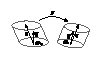
\includegraphics[scale=6.0,trim=0cm 0.2cm 0cm 0cm, clip=true]{Imagens/Cap3/DefArea.eps}	
	\caption{Mudança na área na mudança de configuração.}
	\label{fig:DefArea}
\end{figure}

Considerando a relação da Eq. \eqref{eq:RelVet}, e a arbitrariedade de $\mathbf{u}$, escreve-se a seguinte expressão para relacionar as áreas inicial e atual:

\begin{align}
\mathbf{n}dA = J \mathbf{B} \cdot \mathbf{N} dA_{0}, \label{eq:Nanson}
\end{align}

\noindent com $\mathbf{B} = \gradDeformation^{-t}$. Essa relação é conhecida como Fórmula de Nanson.

\section{Equilíbrio de corpos deformáveis} \label{sec:Equilibrio}

No estudo do equilíbrio de corpos deformáveis a análise da energia mecânica é um assunto de grande importância. A energia mecânica é formada basicamente por três parcelas: energia potencial das forças externas ($\extEnergy$), energia de deformação ($\intEnergy$) e energia cinética ($\kinEnergy$). A energia total mecânica ($\totalEnergy$) é um funcional obtido pela soma dessas três parcelas, sendo escrita da seguinte maneira:

\begin{align}
\totalEnergy = \extEnergy + \kinEnergy + \intEnergy.
\end{align}

O princípio da estacionariedade da energia, define que um corpo quando em equilíbrio apresenta a primeira variação do funcional de energia mecânica nula, sendo o equilíbrio estável quando a posição de equilíbrio representa um mínimo local para a energia mecânica total. O princípio da estacionariedade, utilizando uma descrição das equações de equilíbrio em posições, pode ser expresso matematicamente como:

\begin{align}
\delta\totalEnergy = \frac{\partial{\totalEnergy}}{\partial{\ePosition}} \cdot \delta\ePosition = \mathbf{0}, \label{eq:equilibrio}
\end{align}

\noindent ou, dada a arbitrariedade de $\delta\ePosition$,
\begin{align}
\delta\totalEnergy = \delta\extEnergy + \delta\kinEnergy + \delta\intEnergy.
\end{align}



\subsection{Equações globais de equilíbrio em descrição Euleriana e variação do funcional de energia mecânica}

O sólido da Fig. \ref{fig:EquiSol} está sujeito a forças de corpo $\ebodyLoad$ e forças de superfície $\tractionLoad$, com $\tractionLoad = \stresstensor^{t} \cdot \mathbf{n}$, sendo $\stresstensor$ o tensor de tensões de Cauchy e $ \mathbf{n}$ equivalente ao versor unitário normal a superfície. Aplicando-se a segunda Lei de Newton, considerando que a configuração do meio contínuo apresentada é a atual, chega-se a seguinte expressão que descreve o equilíbrio global do mesmo:

\begin{align}
\int_{V} \ebodyLoad dV + \int_{A} \stresstensor^{t} \cdot \mathbf{n} dA = \int_{V} \rho \solidAccel dV, \label{Eq:forSuper}
\end{align}

\noindent com $\rho$ representando a massa específica do material que compõe o sólido e $\solidAccel$ é a derivada material da velocidade do ponto material (aceleração do corpo).

\begin{figure}[htb!]
	\centering
	\includegraphics[scale=4,trim=0cm 0.2cm 0cm 0cm, clip=true]{Imagens/Cap3/eqSol3.pdf}	
	\caption{Sólido sujeito a um conjunto de carregamento externo.}
	\label{fig:EquiSol}
\end{figure}
 
 Aplicando o teorema de Gauss sobre a Eq.\eqref{Eq:forSuper}, pode-se escrever também as equações de equilíbrio global em descrição Euleriana da seguinte forma:

\begin{align}
\int_{V} \ebodyLoad dV + \int_{V} div({\stresstensor}^{t}) dV = \int_{V} \rho  \solidAccel dV. \label{eq:equilibrioEule}
\end{align}

Baseado na Eq. \eqref{eq:equilibrio} pode-se reescrever a Eq. \eqref{eq:equilibrioEule} como:

\begin{align}
\delta\totalEnergy = \int_{V} \left(- \ebodyLoad -  div({\stresstensor}^{t}) + \rho \solidAccel\right) \cdot \delta\ePosition dV = 0.\label{eq:equilibrioEule2}
\end{align}

Desta forma deve haver uma igualmente entre os termos da Eq. \eqref{eq:equilibrioEule2} e os termos $\delta\extEnergy$, $\delta\kinEnergy$ e $\delta\intEnergy$. Antes de abordar essa relação, o segundo termo de Eq. \eqref{eq:equilibrioEule2} será desdobrado em dois:

\begin{align}
\int_{V} - div({\stresstensor}^{t}) \cdot \delta\ePosition dV = -\int_{A} \tractionLoad \cdot \delta\ePosition dA +  \int_{V}\stresstensor : \divergence_\ePosition \delta\ePosition dV,\label{eq:DivisaoStress}
\end{align}

\noindent ou,
\begin{align}
\int_{V} - div({\stresstensor}^{t}) \cdot \delta\ePosition dV = -\int_{A} \tractionLoad \cdot \delta\ePosition dA +  \int_{V}\stresstensor : \delta\straintensor dV.\label{eq:DivisaoStress2},
\end{align}

\noindent com $\straintensor$ sendo o tensor de deformação de engenharia.

As parcelas de $\delta\extEnergy$, $\delta\kinEnergy$ e $\delta\intEnergy$ são relacionadas aos termos da Eq. \eqref{eq:equilibrioEule2} como:

\begin{align}
\delta\extEnergy = - \int_{V} \ebodyLoad \cdot \delta \ePosition - \int_{A} \tractionLoad \cdot \delta\ePosition dA \\
\delta\kinEnergy = \int_{V} \rho \solidAccel \cdot \delta\ePosition dV\\
\delta\intEnergy = \int_{V}\stresstensor : \delta\straintensor dV.
\end{align}

Dessa forma, uma outra maneira de se expressar as equações global de equilíbrio Euleriano é:

\begin{align}
-\int_{V}  \ebodyLoad \cdot \delta \ePosition dV - \int_{A} \tractionLoad \cdot \delta\ePosition  dA + \int_{V} \rho  \solidAccel \cdot \delta \ePosition  dV + \int_{V}\stresstensor : \delta\straintensor dV = 0. \label{eq:EquilibrioEuleFinal}
\end{align}

A equivalência entre a equação de equilíbrio obtida pela primeira lei de Euler e os termos da variações do potencial de energia mecânica total é apresentada de maneira detalhada em \citeonline{Coda:2018}.

\subsection{Equação da conservação da massa}

A massa pode ser calculada em qualquer instante de tempo ($t$) da análise, e considerando-se que a massa não possa ser retirada ou criada, a equação da conservação da massa ($M$) define que:

\begin{align}
M = \int_{V_{0}} \rho_{0}dV_{0} = \int_{V(t)} \rho(t)dV. \label{eq:conserMassa}
\end{align}

Considerando a Eq.\ref {eq:relVol}, a conservação da massa pode ainda ser expressa como:

\begin{align}
M = \int_{V_{0}} \rho(t) J(t) dV_{0}. \label{eq:conserMassa2}
\end{align}

\subsection{Equações globais de equilíbrio em descrição Lagrangiana}

Partindo-se da Eq. \eqref{Eq:forSuper} do equilíbrio Euleriano, e utilizando as relações para a mudança de volume e área apresentadas nas Eq. \eqref{eq:relVol} e  Eq. \eqref{eq:Nanson} respectivamente, em conjunto com a equação da conservação da massa (Eq. \eqref{eq:conserMassa}), chega-se a:

\begin{align}
\int_{V_{0}} \bodyLoad  dV_{0} + \int_{A_{0}} J \stresstensor^{t} \cdot \mathbf{B} \cdot \mathbf{N} dA_{0} = \int_{V_{0}} \rho_{0} \solidAccel dV_{0}, \label{eq:eqLag1}
\end{align}

\noindent com $\bodyLoad$ sendo as forças de corpo descritas na configuração inicial. Considerando que o tensor das tensões de Piola Kirchhoff de primeira espécie $\mathbf{P}$ é escrito como $\mathbf{P}^{t} = J \stresstensor^{t} \cdot \mathbf{B}$, pode-se rescrever a Eq. \eqref{eq:eqLag1} como:

\begin{align}
\int_{V_{0}} \bodyLoad dV_{0} + \int_{A_{0}} \mathbf{P}^{t} \cdot \mathbf{N} dA_{0} = \int_{V_{0}} \rho_{0} \solidAccel dV_{0}, \label{eq:eqLag2}.
\end{align}

Como consequência a versão da Eq. \eqref{eq:EquilibrioEuleFinal} em descrição Lagrangiana é descrita por:

\begin{align}
-\int_{V_{0}}  \bodyLoad \cdot \delta\ePosition dV_{0} - \int_{A_{0}} \ltractionLoad \cdot \delta\ePosition dA_{0} + \int_{V_{0}} \rho_{0} \solidAccel \cdot \delta\ePosition dV_{0} + \int_{V_{0}} \mathbf{P}^{t} : \delta\gradDeformation dV_{0} = 0. \label{eq:eqLag3},
\end{align}

\noindent com $\ltractionLoad$ sendo as forças de superfície na configuração inicial. 

Seguindo a metodologia de \citeonline{Coda:2018}, deseja-se trabalhar com o segundo tensor de tensões de Piola Kirchhoff ($\piolaStress$), o qual, ao contrário de $\mathbf{P}$, é sempre simétrico. Dessa forma, utiliza-se do fato que:

\begin{align}
\mathbf{P} = \piolaStress^{t} \cdot \gradDeformation,
\end{align}

\noindent escreve-se a equação do equilíbrio Lagrangiano local que será utilizada nas aproximações do MEF:

\begin{align}
-\int_{V_{0}}\bodyLoad \cdot \delta\ePosition dV_{0} - \int_{A_{0}} \ltractionLoad \cdot \delta\ePosition dA_{0} + \int_{V_{0}} \rho_{0} \solidAccel \cdot \delta\ePosition dV_{0} + \int_{V_{0}} \piolaStress : \delta\greenStrain dV_{0} = 0,\label{eq:eqLagFinal}
\end{align}


\subsection{Modelo constitutivo de Saint-Venant-Kirchhoff}

A lei constitutiva hiperelástica de Saint-Venant-Kirchhoff estabelece uma relação linear entre o tensor das tensões de Piola Kirchhoff de segunda espécie e o tensor de deformação de Green, e pode ser escrita pela expressão generalizada da energia de deformação por:

\begin{align}
u_{e}(E) = \frac{1}{2} \greenStrain : \constitutiveTensor : \greenStrain,
\end{align}

\noindent ou, em notação indicial:

\begin{align}
u_{e}(E) = \frac{1}{2} E_{kl} C_{klij} E_{ij}
\end{align}


\noindent com $\constitutiveTensor$ representando o tensor constitutivo elástico isotrópico, que é um tensor de quarta ordem definido como:

\begin{gather}
\constitutiveTensor_{ijkl}=\left(\bulkModulus - \frac{2}{3}\shearModulus \right)\delta_{ij}\delta_{kl} + \shearModulus(\delta_{ik}\delta_{jl}+\delta_{il}\delta_{jk}),
\end{gather}

\noindent sendo $\delta_{ij}$ o delta de Kronocker, $\bulkModulus$ e $\shearModulus$ os módulos volumétrico e de cisalhamento respectivamente, os quais são calculados através das seguintes relações:

\begin{gather}
\bulkModulus=\lameParameter+\frac{2}{3}\shearModulus,\\
\shearModulus=\frac{\elasticModulus}{2(1+\poisonsRatio)},\\
\lameParameter=\frac{\poisonsRatio \elasticModulus}{(1+\poisonsRatio)(1-2\poisonsRatio)},
\end{gather}

\noindent com $\elasticModulus$ sendo o módulo de elasticidade longitudinal e $\poisonsRatio$ o coeficiente de Poisson. Ressalta-se que essa lei constitutiva aqui utilizada é adequada para grandes deslocamentos, entretanto, a mesma não é adequada para grandes deformações.

\section{Método dos Elementos Finitos Posicional}

\subsection{Elemento finito de Casca}

As cascas são sólidos que possuem uma de suas dimensões muito menor do que a outras. A cinemática utilizada para os elementos finitos de casca é aquela apresentada em \citeonline{SanchesC:2010b}, \citeonline{SanchesC:2010a}, na qual aplica-se uma aproximação das configurações do sólido baseada em posições e vetores generalizados como graus de liberdade. A proposta não utiliza o conceito de rotações como graus de liberdade, propiciando um método que conserva o momento angular e linear para grandes deslocamentos de corpo rígido quando utilizado o integrador temporal de Newmark.

As funções que definem a mudança de configuração para a superfície média da casca, conforme pode ser observada na Fig. \ref{fig:casca1}, são definidas como:

\begin{align}
\deformation^{m0} = \lPosition^{m}(\xi_{1},\xi_{2},\mathbf{X}_{l}) = N_{l} (\xi_{1},\xi_{2}) \mathbf{X}_{l}\label{eq:Lposition}\\
\deformation^{m1} = \ePosition^{m}(\xi_{1},\xi_{2},\SolidPos_{l}) = N_{l} (\xi_{1},\xi_{2}) \SolidPos_{l}, \label{eq:Eposition}
\end{align}

\noindent com $\deformation^{m0}$ sendo a função mapeamento da superfície média das coordenadas do domínio paramétrico, definidas por $\bm{\xi}$, para o domínio inicial. Já $\deformation^{m1}$ é a função mapeamento da superfície média do domínio paramétrico para o domínio atual. $\mathbf{X}_{l}$ e $\SolidPos_{l}$ representam as coordenadas do nó $l$ do elemento nas configurações inicial e atual respectivamente, e,  $N_{l}$ representa a função de forma do nó $l$.

\begin{figure}[htb!]
	\centering
	\includegraphics[scale=0.8,trim=0cm 0.0cm 0cm 0cm, clip=true]{Imagens/Cap3/midSurf.pdf}	
	\caption{Mapeamento da superfície média.}
	\label{fig:casca1}
\end{figure}

Para completar a cinemática do casca, as coordenadas inicias e atuais de qualquer ponto da casca podem ser calculadas pela adição às aproximações apresentadas nas Eq. \eqref{eq:Lposition} e Eq. \eqref{eq:Eposition} de vetores posição partindo da superfície média, conforme Fig. \ref{fig:casca2}. Dessa forma pode-se escrever as coordenadas de um ponto como:

\begin{align}
\lPosition &= \lPosition^{m} + \mathbf{v}^{0}\\
\ePosition &= \ePosition^{m} + \mathbf{v}^{1},
\end{align}

\begin{figure}[htb!]
	\centering
	\includegraphics[scale=0.8,trim=0cm 0.0cm 0cm 0cm, clip=true]{Imagens/Cap3/genvec.pdf}	
	\caption{Vetores de posição.}
	\label{fig:casca2}
\end{figure}

\noindent com $\mathbf{v}^{0}$ e $\mathbf{v}^{1}$ sendo os vetores posição para a configuração inicial (perpendicular à superfície média) e atual respectivamente, que são expressos da seguinte forma:

\begin{align}
\mathbf{v}^{0} = \frac{h_{0}}{2}N_{l}\left(\xi_{1},\xi_{2}\right)\mathbf{V}_{l}^{0}\xi_{3},\\
\mathbf{v}^{1} = \frac{h_{0}}{2}N_{l}\left(\xi_{1},\xi_{2}\right)\mathbf{V}_{l}^{1}\left[\xi_{3} + \alpha\left(\xi_{1},\xi_{2}\right)\xi_{3}^2\right],
\end{align}

\noindent com $h_{0}$ representando a espessura média inicial do elemento de casca, $\mathbf{V}_{l}^{0}$ e $\mathbf{V}_{l}^{1}$ o vetor de posição do nó $l$ nas configurações inicial e atual, e $\alpha$ é chamada de taxa linear de variação da espessura e é parametrizada por seus valores nodais $\Lambda_{l}$ da seguinte forma:

\begin{align}
\alpha\left(\xi_{1},\xi_{2}\right) = N_{l}\left(\xi_{1},\xi_{2}\right)\Lambda_{l}.
\end{align}

Por fim, o mapeamento posicional da casca nas configurações inicial e atual é descrito por:

\begin{align}
\deformation^{0} =  N_{l} (\xi_{1},\xi_{2}) \mathbf{X}_{l} + \frac{h_{0}}{2}N_{l}\left(\xi_{1},\xi_{2}\right)\mathbf{V}_{l}^{0}\xi_{3} \label{eq:f0Casca} \\ 
\deformation^{1} =  N_{l} (\xi_{1},\xi_{2}) \SolidPos_{l} +  \frac{h_{0}}{2}N_{l}\left(\xi_{1},\xi_{2}\right)\mathbf{V}_{l}^{1}\left[\xi_{3} + \alpha\left(\xi_{1},\xi_{2}\right)\xi_{3}^2\right]. \label{eq:f1Casca}
\end{align}

As equações Eq. \eqref{eq:f0Casca} e Eq. \eqref{eq:f1Casca} apresentam sete parâmetros incógnitos em cada nó $l$: 3 posições ($ \SolidPos_{l}$), 3 componentes do vetor generalizado ($\mathbf{V}_{l}^{1}$) e o valor nodal da variação linear da deformação na espessura $\Lambda_{l}$. A partir desse ponto os parâmetros incógnitos serão descritos por uma única variável $ \SolidPos_{l}^{i}$, com $i = 0,1$ e $2$ representando as posições, $i = 3,4$ e $5$ as componentes do vetor generalizado e $i = 6$ a taxa de variação linear da espessura.


Para iniciar-se a descrição do MEF posicional, adiciona-se mais um termo à Eq. \eqref{eq:eqLagFinal} respectivo a forças concentradas nodais e fica-se com a seguinte definição para as equações de equilíbrio Lagrangiana:

\begin{align}
-\mathbf{F}_{l}\delta\SolidPos_{l} - \int_{V_{0}}\bodyLoad \cdot \delta\ePosition dV_{0} - \int_{A_{0}} \ltractionLoad \cdot \delta\ePosition dA_{0} + \int_{V_{0}} \rho_{0} \solidAccel \cdot \delta\ePosition dV_{0} + \int_{V_{0}} \piolaStress : \delta\greenStrain dV_{0} = 0,
\end{align}

\noindent sendo o termo $-\mathbf{F}_{l}$ respectivo a força concentrada aplicada sobre o nó $l$. O tensor $\greenStrain = \greenStrain (\SolidPos)$ é função de $\gradDeformation$, e pode ser obtido em função das posições através de $\deformation^{0} $ e $\deformation^{1} $ como:

\begin{align}
\gradDeformation = \gradDeformation^{1}\left(\gradDeformation^{0}\right)^{-1} \label{eq:gradDeformation}.
\end{align}

Considerando uma aproximação tradicional das variáveis de elementos finitos, tem-se:

\begin{align}
\delta\ePosition = N_{l} (\xi_{1},\xi_{2})\delta\SolidPos_{l},\\
\bodyLoad = N_{l} (\xi_{1},\xi_{2}) \mathbf{B}_{l}^{0},\\
\ltractionLoad = N_{l} (\xi_{1},\xi_{2}) \mathbf{Q}_{l}^{0},\\
\solidAccel = N_{l} (\xi_{1},\xi_{2}) \mathbf{\ddot{Y}}_{l},
\end{align}

\noindent da arbitrariedade de $\delta\SolidPos$ as equações do equilíbrio em função das posições nodais são escritas como:

\begin{align}
\begin{split}
&-\mathbf{F}_{l} - \int_{V_{0}^{el}}N_{m} (\coordAdimen)N_{l} (\coordAdimen)dV_{0}^{el} \mathbf{B}_{m}^{0} -\int_{A_{0}^{el}}N_{m} (\coordAdimen)N_{l} (\coordAdimen)dA_{0}^{el} \mathbf{Q}_{m}^{0}  \\& + \int_{V_{0}^{el}}\rho_{0} N_{m} (\coordAdimen)N_{l} (\coordAdimen)dV_{0}^{el} \mathbf{\ddot{Y}}_{m} + \int_{V_{0}^{el}} \piolaStress : \frac{\partial\greenStrain}{\partial\SolidPos_{l}}dV_{0}^{el}.
\end{split}
\end{align}

\subsection{Integração temporal e técnica de solução}

As equações do equilíbrio baseadas em posição podem ser apresentadas sinteticamente como:

\begin{align}
\frac{\partial\totalEnergy}{\partial\SolidPos} = \frac{\partial\extEnergy}{\partial \SolidPos} + \frac{\partial\kinEnergy}{\partial \SolidPos} + \frac{\partial\intEnergy}{\partial \SolidPos} = \mathbf{0},
\end{align}
  
\noindent ou ainda,

\begin{align}
 - \concLoad^{ext}(t) + \solidMass\SolidAccel_{}+ \concLoad^{int}(\SolidPos) + \solidDamping\SolidVel_{} = \mathbf{0}, \label{eq:Equilibrio}
\end{align}

\noindent na qual $ \concLoad^{int}(\SolidPos)$ representa as forças internas provenientes da variação da energia potencial interna, $\solidMass$ é a conhecida como matriz de massa proveniente da variação da energia cinética e $\mathbf{F}^{ext}$ representam as forças externas na estrutura fruto da variação da energia potencial das forças externas. O termo $\solidDamping$ representa uma matriz de amortecimento proporcional a massa, e $\SolidVel_{}$ a velocidade nodal.

A integração temporal das equações apresentadas na Eq. \eqref{eq:Equilibrio} inicia-se com a discretização temporal do tempo de maneira que:

\begin{align}
t_{n+1} = t_{n} + \Delta t, \label{eq:disTime}
\end{align}

\noindent na qual $t_{n+1}$ representa o tempo no instante atual, $t_{n}$ o instante de tempo anterior e  $\Delta t$ o intervalo de tempo utilizado na discretização. Utilizando as aproximações de Newmark, posições, velocidade e aceleração nos tempos $n+1$ e $n$ são relacionados por:

\begin{gather}
\SolidPos_{n+1}=\SolidPos_{n} + \timeStep \SolidVel_{n}+\left(\frac{1}{2}-\beta\right) \timeStep^2 \SolidAccel_{n}+ \beta \timeStep^2 \SolidAccel_{n+1},\label{eq:newmark1}\\
\SolidVel_{n+1} = \SolidVel_{n}+(1-\gamma)\timeStep \SolidAccel_{n}+\gamma \timeStep \SolidAccel_{n+1},\label{eq:newmark2}
\end{gather}

\noindent em que $\beta$ e $\gamma$ são parâmetros dependentes do comportamento assumido para a aceleração, adotados nesse trabalho como $\gamma=\sfrac{1}{2}$ e $\beta=\sfrac{1}{4}$ para uma aceleração constante.

Considerando a discretização temporal apresentada em Eq. \eqref{eq:disTime} e aplicando-se a Eq. \eqref{eq:newmark1} e Eq. \eqref{eq:newmark2} à Eq. \eqref{eq:Equilibrio} de maneira a escrever-se a equação somente em função das posições nodais, tem-se, para um instante $n+1$ a seguinte relação:

\begin{gather}
\concLoad^{int}_{n+1}- \concLoad^{ext}_{n+1} + \frac{\solidMass}{\beta \timeStep^2} \SolidPos_{n+1}-\solidMass \mathbf{Q}_n+ \solidDamping\mathbf{R}_n + \frac{\gamma \solidDamping}{\beta \timeStep}\SolidPos_{n+1} - \gamma\timeStep \solidDamping\mathbf{Q}_n = \mathbf{0},
\label{eq:equilibrio_newmark}
\end{gather}

\noindent em que $\mathbf{Q}_n$ e $\mathbf{R}_n$ representam os termos dependentes apenas de velocidades, acelerações e posições do instante anterior, dados por:

\begin{gather}
\mathbf{Q}_n = \frac{\SolidPos_n}{\beta \timeStep^2} + \frac{\SolidVel_n}{\beta \timeStep} + \left(\frac{1}{2\beta} -1 \right)\SolidAccel_n,\label{eq:Qn}\\
\mathbf{R}_n = \SolidVel_n+\timeStep(1-\gamma)\SolidAccel_n.\label{eq:Rn}
\end{gather}


Pode-se escrever ainda o problema não linear definido por
\eqref{eq:equilibrio_newmark} em função do resíduo da equação governante
discretizada no espaço e no tempo, tal que:

\begin{gather}
%\begin{dcases}
\NNSS\left(\SolidPos_{n+1}\right) = \concLoad^{int}_{n+1}- \concLoad^{ext}_{n+1} + \frac{\solidMass}{\beta \timeStep^2} \SolidPos_{n+1}-\solidMass \mathbf{Q}_n+ \solidDamping\mathbf{R}_n + \frac{\gamma \solidDamping}{\beta \timeStep}\SolidPos_{n+1} - \gamma\timeStep \solidDamping\mathbf{Q}_n= \zeroMatrix.
%\end{dcases}
\label{eq:equilibrio_newmark1.5}
\end{gather}

O problema não linear da Eq. \eqref{eq:equilibrio_newmark1.5} é resolvido por meio do método iterativo de Newton-Raphson. Para isso, realiza-se uma expansão em série de Taylor de primeira ordem:

\begin{gather}
\NNSS\left(\SolidPos_{n+1}^{i+1}\right) \approx \NNSS\left(\SolidPos_{n+1}^{i}\right) + \Delta\NNSS\left(\SolidPos_{n+1}^{i}\right)\Delta\SolidPos_{i} 
\end{gather}

\noindent em que $i$ indica o índice da iteração atual. Na primeira iteração para o cálculo de $\SolidPos_{n+1}$ utiliza-se como predição da iteração anterior os valores das variáveis no passo de tempo $n$. O método de Newton-Raphson consiste em resolver o seguinte sistema:

\begin{gather}
\Delta\NNSS\left(\SolidPos_{n+1}^{i}\right)\Delta\SolidPos^{i} = -\NNSS\left(\SolidPos_{n+1}^{i}\right) \label{eq:NR}
\end{gather}

\noindent com:

\begin{gather}
\Delta\NNSS\left(\SolidPos_{n+1}^{i}\right) = \frac{\partial^{2}\totalEnergy}{\partial\SolidPos^{2}} = \frac{\partial^{2}\intEnergy}{\partial \SolidPos^{2}} + \frac{\solidMass}{\beta \timeStep^2} + \frac{\gamma \solidDamping}{\beta \timeStep}.
\end{gather}

A cada iteração de Newton-Raphson atualiza-se a posição, a aceleração e a velocidade de acordo com as seguintes equações:

\begin{gather}
\SolidPos_{n+1}^{i+1} = \SolidPos_{n+1}^{i} + \Delta\SolidPos^{i} \label{UD1}\\
\SolidAccel_{n+1}^{i+1} = \frac{\SolidPos_{n+1}^{i+1}}{\beta \timeStep^2} + \mathbf{Q}_n  \label{UD2} \\
\SolidVel_{n+1}^{i+1} = \frac{\gamma \SolidPos_{n+1}^{i+1}}{\beta \timeStep} + \mathbf{R}_n - \gamma\Delta t \mathbf{Q}_n  \label{UD3}
\end{gather}


\subsection{Implementação Computacional}

Emprega-se o programa para análise não linear de estruturas de casca cedido pelo professor Humberto Breves Coda \cite{CodaP:2007,CodaP:2008}, o qual segue a formulação descrita neste texto e é implementado em linguagem FORTRAN, com paralelização em protocolo MPI.

O algoritmo implementado foi criteriosamente estudado de forma a permitir a implementação do acoplamento, sendo apresentado em Alg. \ref{alg:solid_temporalIntegration}.


\begin{algorithm}
	\caption{Algoritmo para problemas de dinâmica dos sólidos computacional}
	\label{alg:solid_temporalIntegration}
	\begin{algorithmic}[1]
		\For {o passo de tempo $0$ até \timeInterval} 
		\State $i=0$;
		\State Predição da solução: 
		\begin{align}
		\SolidPos_{n+1}^{0} = \SolidPos_{n},\\
		\SolidVel_{n+1}^{0} = \SolidVel_{n},\\
		\SolidAccel_{n+1}^{0} = \SolidAccel_{n};
		\end{align}
		\State Calcula-se  nível de força aplicado $\concLoad^{ext}_{n+1}(t_{n+1})$ e/ou as posições prescritas $\SolidPos_{n+1}$;
		\State Calculam-se os valores de $\mathbf{Q}_n$ (Eq. \eqref{eq:Qn}) e $\mathbf{R}_n$ (Eq. \eqref{eq:Rn});
		\While{($\epsilon$ < tolerância)}
		\State $i$++;
		\State Cálculo do incremento da variável do problema: $\SolidPos_{n+1}^{i}$ de acordo com a Eq. \eqref{eq:NR};
		\State Atualização da solução: calculada de acordo com Eq. \eqref{UD1}, Eq. \eqref{UD2} e Eq. \eqref{UD3}.
		\State Cálculo do erro:
		\begin{align}
		\epsilon = \lVert \Delta\NNSS\left(\SolidPos_{n+1}^{i+1}\right) \lVert_{L^2} 
		\end{align}
		ou,
		\begin{align}
		\epsilon = \lVert\Delta\SolidPos_{n+1}^{i+1}\lVert_{L^2} 
		\end{align}
		\EndWhile
		\EndFor
	\end{algorithmic}
\end{algorithm}

\section{Exemplo de aplicação - Casca cilíndrica com \textit{snap through} dinâmico}

Nesta seção é apresentada uma simulação feita com o código cedido pelo professor Humberto Breves Coda para problemas de análise não-linear geométrica de cascas. Esta análise foi realizada com o objetivo de estudar o programa a ser empregado na pesquisa.

O problema clássico analisado trata-se de um casca cilíndrica submetida a um carregamento concentrado em seu centro geométrico. Proposto inicialmente no trabalho de \cite{KuhlR:1999}, o problema apresenta grande não-linearidade geométrica devido ao efeito de \textit{snap-through}. 

A geometria do problema em questão é apresentada na Fig. \ref{fig:CascaGeo}, sendo a espessura da casca equivalente a 0,1 m. Como condições de contorno, têm-se o deslocamento restrito nas direções $x,y,z$ para as bordas retas que formam a geometria da casca. A malha de elementos finitos que representa a superfície média da casca utilizada pode ser visualizada na Fig. \ref{fig:CascaMalha}, a qual é composta por 32 elementos cúbicos e 49 nós. 

\begin{figure}[!htb]
	\centering
	\subfloat[\label{fig:CascaGeo} Malha Local.]{\includegraphics[scale=0.2, trim=0cm 0cm 15cm 0cm, clip=true]{Imagens/Cap3/lateral.pdf}} 
	\subfloat[\label{fig:CascaMalha} Malha Global ]{\includegraphics[scale=0.18,trim=0cm 0cm 15cm 0cm, clip=true]{Imagens/Cap3/teste.pdf}}
	\caption{Casca: Geometria e Malha.}
	\label{fig:Casca}
\end{figure}

O carregamento $P(t)$ é aplicado linearmente no intervalo $t=0s$ até $t=0,2s$, com $P(0)=0kN$ e $P(2s) = 50000kN$, e então mantido constante. As características físicas do material utilizado são: $\elasticModulus = 200GPa$, $\poisonsRatio = 0,25$ e $\rho = 10000 kg/m^3$ e o passo de tempo adotado na simulação é $\Delta_{t} = 0,001s$.

O deslocamento vertical do nó central da casca pode ser visualizado na Fig. \ref{fig:CascaDeslocamento}. O resultado obtido está de acordo com os resultados de \citeonline{ArgyrisPM:2003}, conforme pode ser visto na Fig. \ref{fig:CascaDeslocamentoReferencia} e o campo de deslocamentos nos instantes $t = 0s$, $t = 100ms$ e $t = 155ms$ são apresentados na Fig. \ref{fig:CamposDeslocamentos}.

Embora a implementação do programa de cascas não seja objetivo deste trabalho, e essa análise tenha objetivo de estudar o código a ser empregado, ela também traz indício da robustez e precisão da formulação escolhida.

\begin{figure}[!htb]
	\centering
	\subfloat[\label{fig:CascaDeslocamento} Presente trabalho.]{\includegraphics[scale=.8, trim=0cm 0cm 0cm 0cm, clip=true]{Imagens/Cap3/snap_casca.eps}} \\
	\subfloat[\label{fig:CascaDeslocamentoReferencia} Referência ]{\includegraphics[scale=0.25,trim=0cm 0cm 0cm 0cm, clip=true]{Imagens/Cap3/referencia.png}}\\
	Fonte: \citeonline{ArgyrisPM:2003}
	\caption{Casca: Deslocamento vertical nó central.}
	\label{fig:CascaDeslocamentoT}
\end{figure}


\begin{figure}[!htb]
	\centering
	\subfloat[\label{fig:C0} $t = 0s$.]{\includegraphics[scale=0.08, trim=4cm 15cm 4cm 15cm, clip=true]{Imagens/Cap3/0ms.png}} 
	\subfloat[\label{fig:C1} $t = 100ms$ ]{\includegraphics[scale=0.08,trim=4cm 15cm 4cm 15cm, clip=true]{Imagens/Cap3/100ms.png}}\\
	\subfloat[\label{fig:C2} $t = 155ms$ ]{\includegraphics[scale=0.08,trim=4cm 15cm 4cm 15cm, clip=true]{Imagens/Cap3/155ms.png}}\\
	{\includegraphics[scale=0.3,trim=0cm 0cm 0cm 0cm, clip=true]{Imagens/Cap3/legenda.png}}
	\caption{Casca: Campo de deslocamento.}
	\label{fig:CamposDeslocamentos}
\end{figure}




% \section{Validação e aplicações}
%\textcolor{red}{voltamos a esse ponto se houver tempo...}
% \subsection {Exemplo}

\end{document}